\chapter{Fabrication techniques}
\label{sec:Fabrication}

This chapter presents MTJ stack used for the experiment and describes the complete fabrication process of the sample.

\section{MTJ stack deposition} \label{sec:FabricationStack}

    Based on previous experiments \cite{skowronski2017understanding}, an MTJ layer structure with PMA was proposed and deposited by Singulus AG using TIMARIS sputtering system in $Ar$ atmosphere on an oxidised $Si$ substrate. The substrate was etched before the deposition using ion etching, in order to clean the surface. The layer structure is presented in Tab. \ref{tab:FabricationLayerStructure}. 
    
    Layers 37-35 form a buffer, which reduces the surface roughness and induces proper crystal growth of other layers \cite{banasik2015magnetic}. Layers 34-8 form a SAF, with a reference layer (10-8) on the top. $Co/Pt$ layers 34-21 form a superlattice with strong PMA (Sec. \ref{sec:PrinciplesAdditionalPerpendicular}) which is coupled antiferromagnetically to another $Co/Pt$ superlattice (19-12) through a \SI{0.8}{\nano\meter} $Ru$ spacer (20). A composite reference layer (10-8) is also coupled through thin W layer (which, in addition, serves as a texture break), completing the SAF. A \SI{0.89}{\nano\meter} thick $MgO$ is used as a tunnel barrier (7), which results in the resistance area (RA) product of around \SI{20}{\ohm\times\micro\metre\squared}. Above, a composite free layer is placed (6-4). An important part of the top capping (3-1) is another $MgO$ layer (3), which increases PMA of the free layer.
    
    After the deposition process the sample was annealed at \SI{380}{\celsius} for \SI{60}{\minute}. The process allowed to relax interface stresses of the layers.
    
    \begin{table}[H]
    	\caption{Layer structure of the sample used for experiment, from top to bottom.}
    	\label{tab:FabricationLayerStructure}

    	\begin{center}
    	  \begin{tabular}{r r l l@{\hspace{20pt}} l}
    	    No. & Material & \multicolumn{3}{l}{Thickness (\SI{}{\nano\meter})} \\ \hline
    	    1 & $Ru$ 	& \cellcolor{capping}5.00 & \rdelim\}{3}{3mm}[Top capping] \\
    	    2 & $Ta$ 	& \cellcolor{capping}3.00 \\
    	    3 & $MgO$ 	& \cellcolor{capping}1.00 \\ \hline
    	    4 & $CoFeB$ & \cellcolor{ferromagnetic}0.50 & \rdelim\}{3}{3mm}[Free layer] \\
    	    5 & $W$ 	& \cellcolor{ferromagnetic}0.30 \\
    	    6 & $CoFeB$ & \cellcolor{ferromagnetic}1.30 \\ \hline
    	    7 & $MgO$	& \cellcolor{barrier}0.89 & Tunnel barrier \\ \hline
    	    8 & $CoFeB$ & \cellcolor{ferromagnetic}1.00 & \rdelim\}{3}{3mm}[Reference layer] & \rdelim\}{13}{3mm}[SAF] \\
    	    9 & $W$		& \cellcolor{ferromagnetic}0.25 \\
    	    10& $Co$	& \cellcolor{ferromagnetic}0.90 \\
    	    11& $Ta$	& \cellcolor{ferromagnetic}0.15 \\
    	    12& $Pt$	& \cellcolor{ferromagnetic}0.20 \\
    	   \ldelim\{{2}{3mm}[13\textasciitilde 18]& $Co$ & \cellcolor{ferromagnetic}0.50 & \rdelim\}{2}{3mm}[$\times 3$] \\
    	    &   $Pt$	& \cellcolor{ferromagnetic}0.20 \\
    	    19& $Co$	& \cellcolor{ferromagnetic}0.60 \\
    	    20& $Ru$	& \cellcolor{ferromagnetic}0.80 \\
    	    21& $Co$	& \cellcolor{ferromagnetic}0.60 \\
    	    \ldelim\{{2}{3mm}[22\textasciitilde 33] & $Pt$ & \cellcolor{ferromagnetic}0.20 & \rdelim\}{2}{3mm}[$\times 6$] \\
    	    &   $Co$	& \cellcolor{ferromagnetic}0.50 \\
    	    34& $Pt$	& \cellcolor{ferromagnetic}1.50 \\ \hline
    	    35& $Ta$	& \cellcolor{bottom}0.70 & \rdelim\}{3}{3mm}[Bottom buffer] \\
    	    36& $Ru$	& \cellcolor{bottom}7.00 \\
    	    37& $Ta$	& \cellcolor{bottom}2.00 \\ \hline
    	    & $SiO_2$ & \cellcolor{substrate} & \rdelim\}{2}{3mm}[Oxidised substrate]\\
    	    & $Si$ & \cellcolor{substrate} \\
    	  \end{tabular}
    	\end{center}
    \end{table}

\section{MTJ nanostructurization} \label{sec:FabricationMask}

    To conduct the experiment, and check the behaviour of serially connected storage elements, nanostructurization was done, as effects presented in Sec. \ref{sec:Principles} take place only when the size of the junction is small enough. During the process, MTJs, vias, electrical contacts and connections were fabricated, as described below in Sec. \ref{sec:FabricationFabrication}.
    
    The mask used for the process is presented in Fig. \ref{FabricationMaskAll}.
    
    \begin{figure}[H]
        \centering
        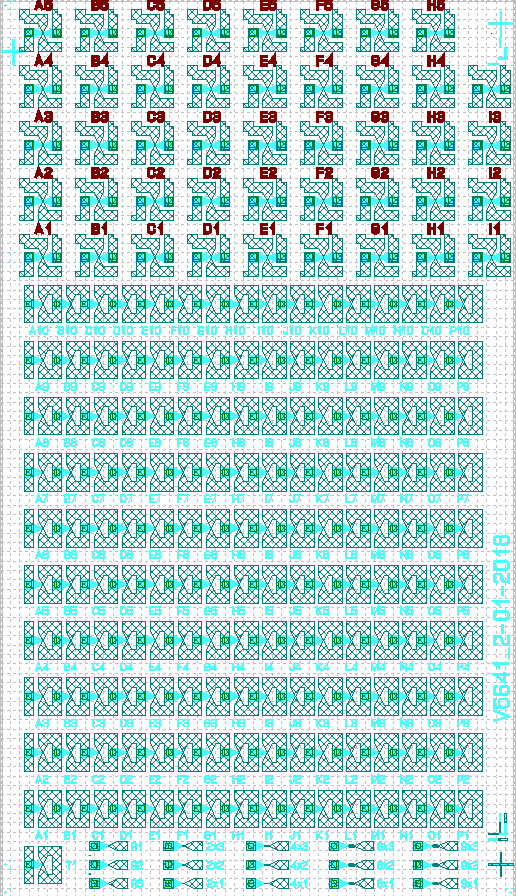
\includegraphics[width=0.4\paperwidth, angle=-90]{img/04/mask_all.png}
        \caption{The overview of the mask used for nanostructurization process.}
        \label{FabricationMaskAll}
    \end{figure}
    
    The mask is divided into four regions:
    
    %noitemsep, 
    \begin{itemize}[noitemsep,label=\textbullet]
    	\item Individual elements for separate storage elements characterization (top, Fig. \ref{FabricationMaskDeta}).
    	\item Storage elements connected in series of 16 with separate access to each storage element, that allows testing different numbers of elements connected in series, and also gives the possibility to deal with malfunctioning elements (middle, Fig. \ref{FabricationMaskDetb}) 
    	\item Miniaturised series connections of 2, 4, 8 and 9 storage elements without separate access (bottom right, Fig. \ref{FabricationMaskDetc})
    	\item Structures prepared for testing resistance of vias and scanning electron microscopy (SEM) imaging during the fabrication process (bottom left, close-up not presented).
    \end{itemize}
    
    All the MTJ devices were fabricated as cylinders with nominal diameter of \SI{100}{\nano\meter}. During the process, after forming of the pillar (Fig. \ref{FabricationPillarEtching}), a SEM image was taken (Fig. \ref{FabricationPillarSEM}) to verify the diameter of the pillar obtained - \SI{130}{\nano\meter}. The difference from the intended size is normal for the process used, and originates from slight overexposure of the photo-resist. All elements were equipped with \SI[product-units = power]{100 x 100}{\micro\meter} raster contact pads. Optical microscope images of the sample after complete nanostructurization are presented in Fig. \ref{FabricationSampDet}. After the fabrication the sample was ready for the measurement process.

\begin{figure}
    \centering
    \begin{subfigure}[b]{0.35\paperwidth}
    	\centering
        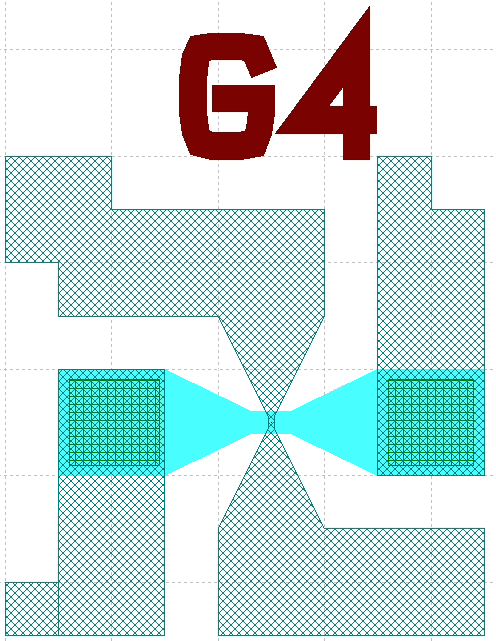
\includegraphics[width=0.15\paperwidth]{img/04/mask_single.png}
        \caption{Single storage element with contacts for testing.}
        \label{FabricationMaskDeta}
    \end{subfigure}
    ~ %add desired spacing between images, e. g. ~, \quad, \qquad, \hfill etc. 
      %(or a blank line to force the subfigure onto a new line)
    \begin{subfigure}[b]{0.35\paperwidth}
    	\centering
        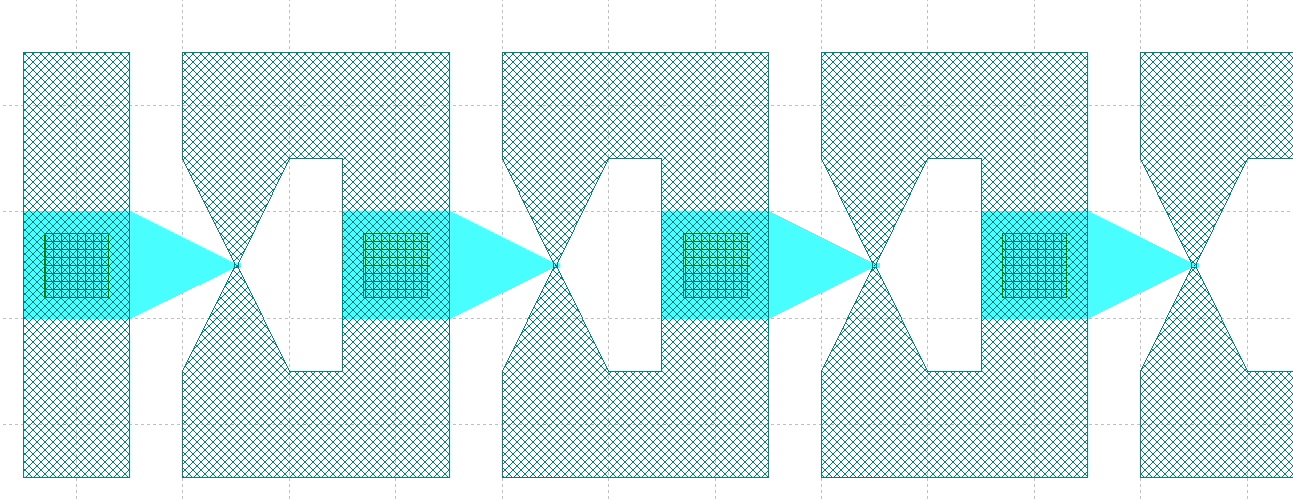
\includegraphics[width=0.3\paperwidth]{img/04/mask_series_big.png}
        \caption{Storage elements connected in series.}
        \label{FabricationMaskDetb}
    \end{subfigure}
    \\
    \begin{subfigure}[b]{0.5\paperwidth}
    	\centering
        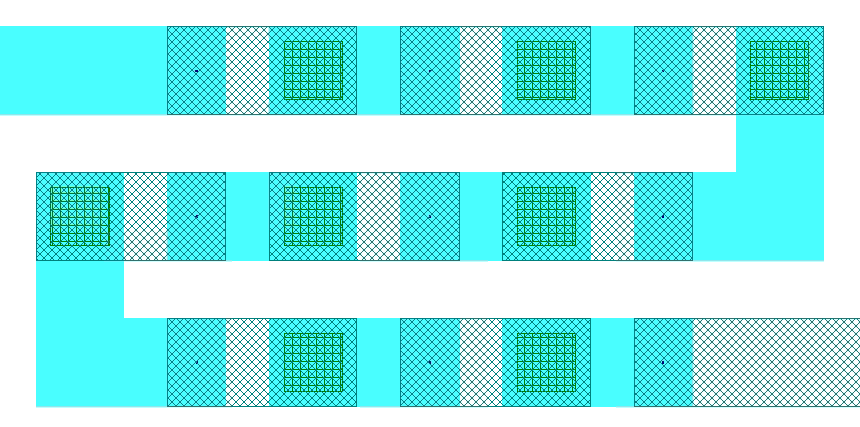
\includegraphics[width=0.3\paperwidth]{img/04/mask_series_9_zoom.png}
        \caption{Miniaturised serial connection of 9 storage elements.}
        \label{FabricationMaskDetc}
    \end{subfigure}
    \caption{Close-ups of different parts of the mask. Scale is not the same for each element.}
    \label{FabricationMaskDet}
\end{figure}

\begin{figure}
    \centering
    \begin{subfigure}[b]{0.35\paperwidth}
    	\centering
        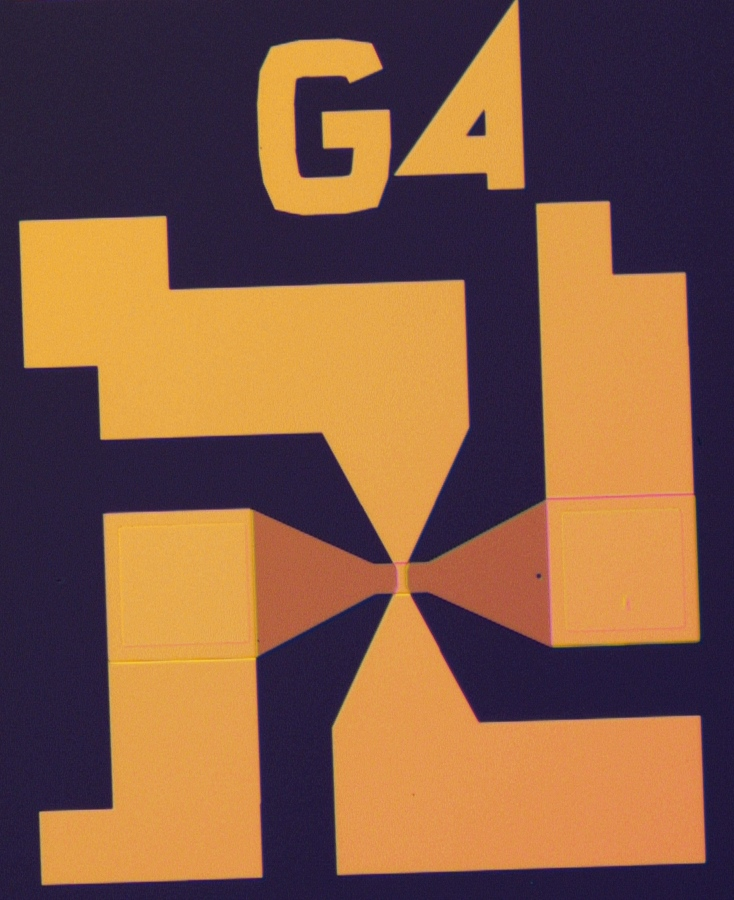
\includegraphics[width=0.15\paperwidth]{img/04/fab_single.jpg}
        \caption{Single storage element with contacts for testing.}
        \label{FabricationSampDeta}
    \end{subfigure}
    ~ %add desired spacing between images, e. g. ~, \quad, \qquad, \hfill etc. 
      %(or a blank line to force the subfigure onto a new line)
    \begin{subfigure}[b]{0.35\paperwidth}
    	\centering
        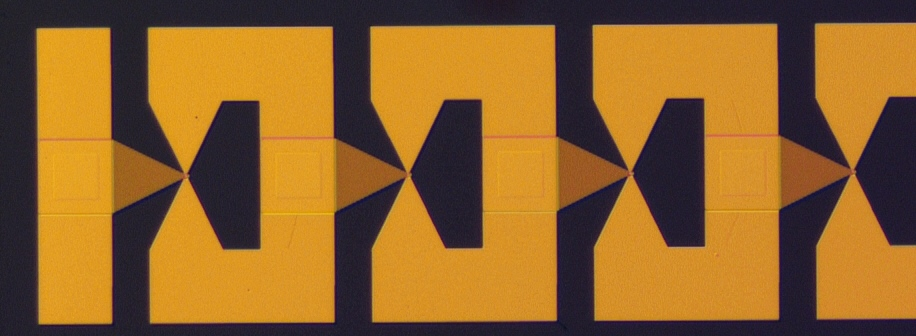
\includegraphics[width=0.3\paperwidth]{img/04/fab_series_big.jpg}
        \caption{Storage elements connected in series.}
        \label{FabricationSampDetb}
    \end{subfigure}
    \\
    \begin{subfigure}[b]{0.5\paperwidth}
    	\centering
        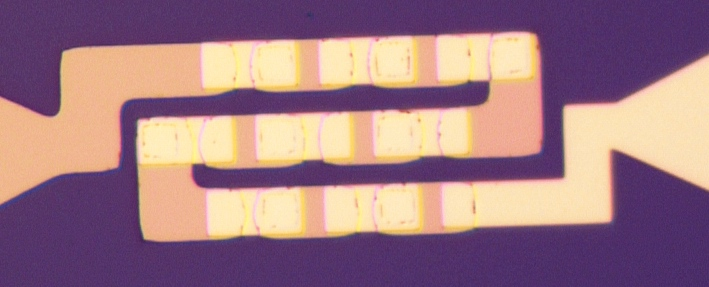
\includegraphics[width=0.3\paperwidth]{img/04/fab_series_9_zoom.jpg}
        \caption{Miniaturised serial connection of 9 storage elements.}
        \label{FabricationSampDetc}
    \end{subfigure}
    \caption{Close-ups of different parts of the sample. Scale is not the same for each element.}
    \label{FabricationSampDet}
\end{figure}

    \begin{figure}[H]
        \centering
        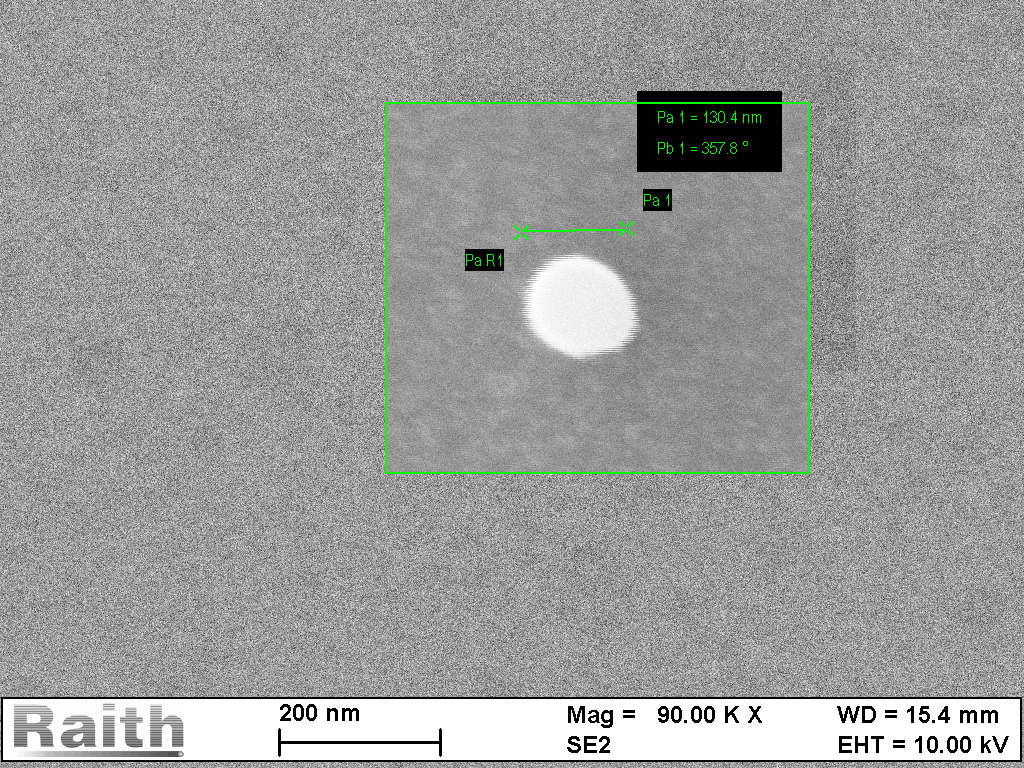
\includegraphics[width=0.75\paperwidth]{img/04/PillarSEM.png}
        \caption{SEM image of the cylindrical storage element. The diameter was determined to be approximately \SI{130}{\nano\meter}.}
        \label{FabricationPillarSEM}
    \end{figure}
    
\section{Fabrication} \label{sec:FabricationFabrication}

    Layers forming MTJ, together with bottom buffer and top capping are deposited by Singulus AG on an oxidised silicon substrate (Figs. \ref{FabricationSubstrate}-\ref{FabricationStack}). These processing steps are performed by the company, because very precise control of deposition conditions are required to obtain correct crystalline structure, and finally a working MTJ. The deposition process is far beyond the scope of this thesis.
    
    Further processing is performed in the Academic Center of Materials and Nanotechnology (ACMiN AGH). In subsequent steps:
    \begin{itemize}[noitemsep,label=\textbullet]
    	\item the bottom electrode is being formed (Figs. \ref{FabricationBottomResist}-\ref{FabricationBottomEtching})
    	\item the insulation is applied, to prevent forming unwanted connections during further processing (Figs. \ref{FabricationBottomOxide}-\ref{FabricationBottomLiftOff})
    	\item pillars and vias are formed and the insulation oxide is applied (Figs. \ref{FabricationPillarResist}-\ref{FabricationPillarLiftOff})
    	\item top electrode is formed, including measurement contacts and connections between MTJ pillars (Figs. \ref{FabricationTopResist}-\ref{FabricationComplete})
    	%\item (Figs. \ref{}-\ref{})
    \end{itemize}
    
\begin{multicols}{2}[]

	\begin{figure}[H]
        \centering
        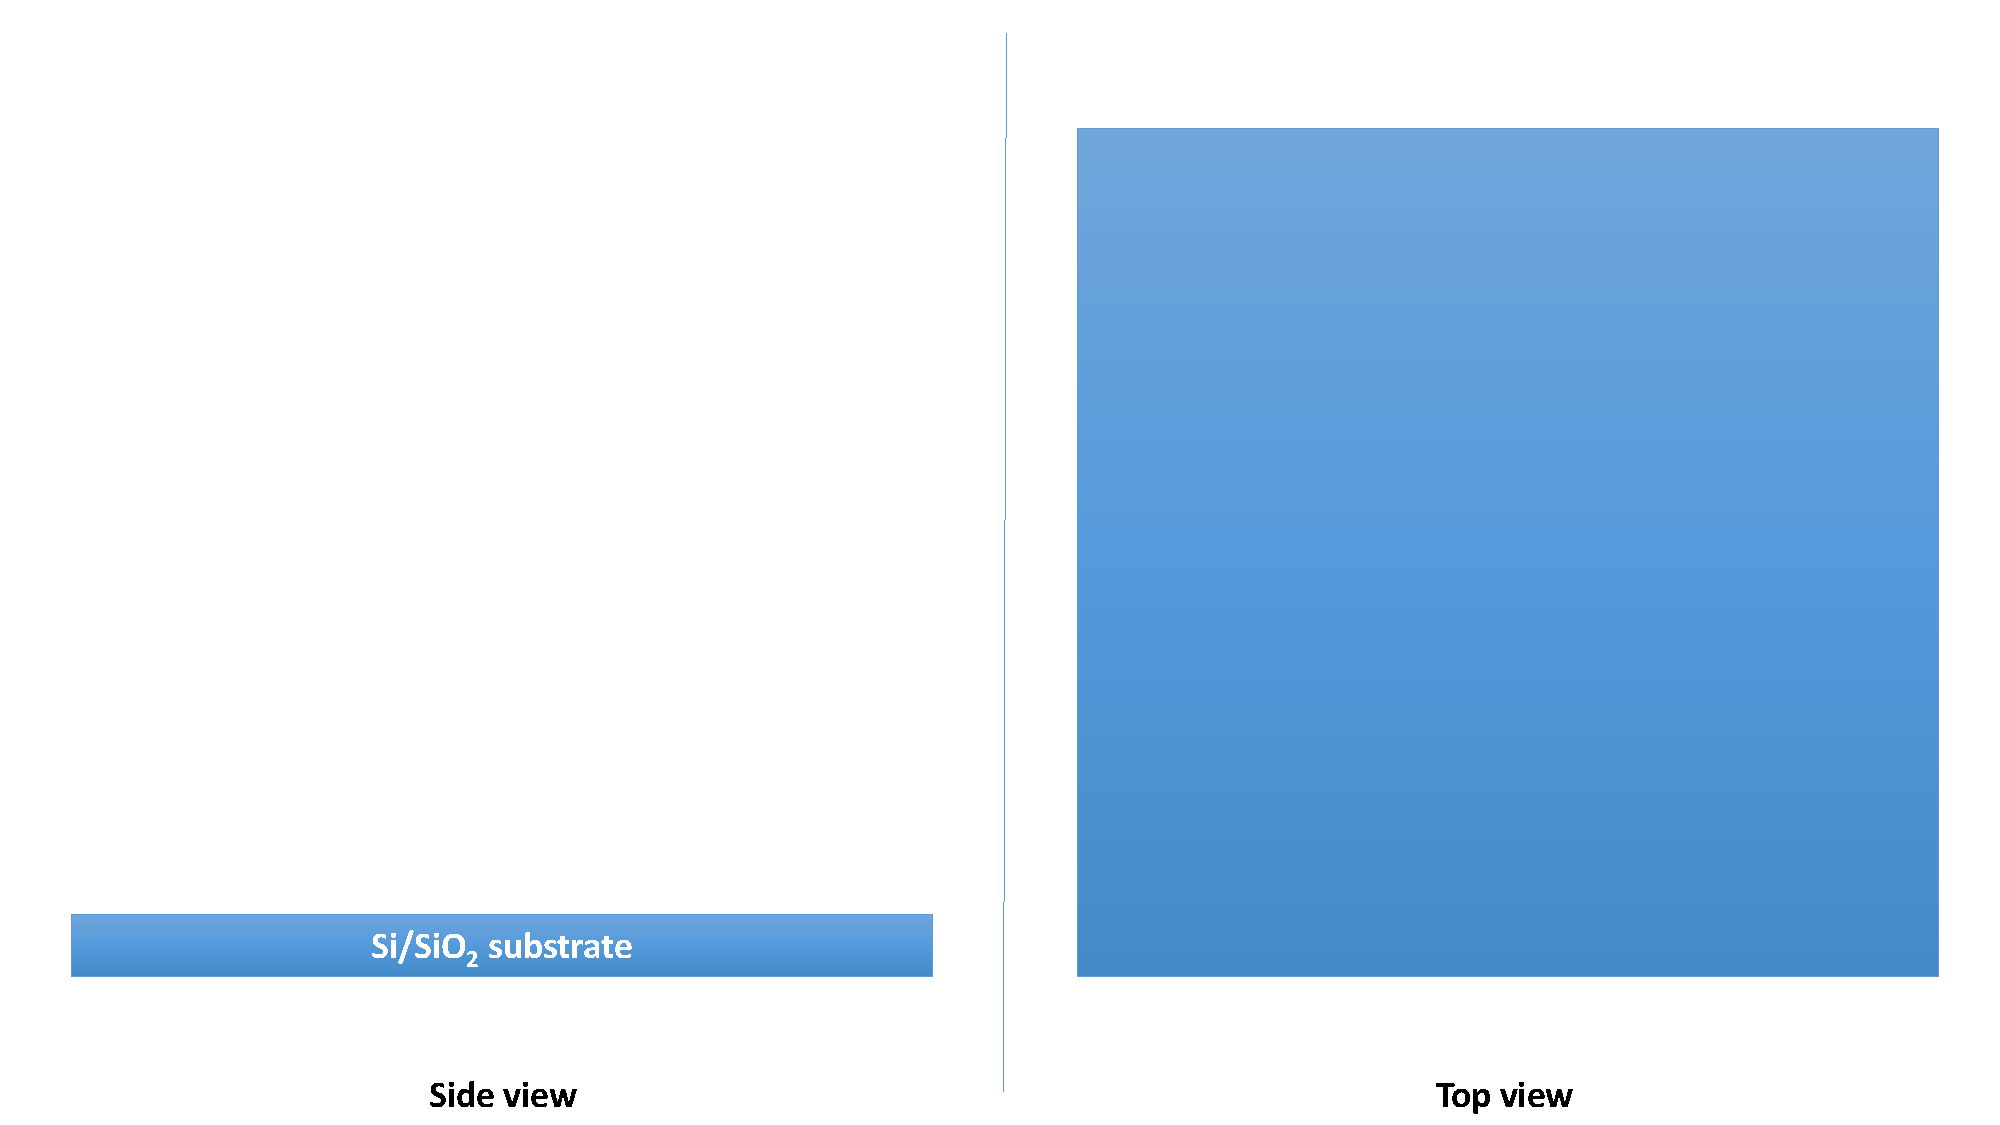
\includegraphics[width=0.375\paperwidth, page=1]{img/04/Manufacturing_under.pdf}
        \caption{A polished and (if required) oxidised silicon wafer is prepared for processing. Size/thickness in this and the following figures are not to scale.}
        \label{FabricationSubstrate}
    \end{figure}
    
	\begin{figure}[H]
        \centering
        \includegraphics[width=0.375\paperwidth, page=2]{img/04/Manufacturing_under.pdf}
        \caption{A thin film of target material is deposited by means of magnetron sputtering. Optionally, an oxygen flow may be provided in order to deposit target material oxide (e.g. $MgO, Al_2O_3$).}
        \label{FabricationSputtering}
    \end{figure}
    
\end{multicols}
\vfill
\begin{multicols}{2}[]
    
    \begin{figure}[H]
        \centering
        \includegraphics[width=0.375\paperwidth, page=3]{img/04/Manufacturing_under.pdf}
        \caption{Requested layer stack with metallic bottom buffer and capping layer is deposited by means of magnetron sputtering. This process is conducted by Singulus AG, as conditions of deposition are crucial for correct crystallization, and therefore, operation of the MTJ. The sample is annealed to recrystallize all layers.}
        \label{FabricationStack}
    \end{figure}
    
    \begin{figure}[H]
        \centering
        \includegraphics[width=0.375\paperwidth, page=4]{img/04/Manufacturing_under.pdf}
        \caption{A negative photo-resist (AR-N 7720.30) is applied in spin-coater at \SI{6000}{\rpm}, resulting in thickness of approx. \SI{1.24}{\micro\meter}. Then the sample is baked for \SI{120}{\second} at \SI{85}{\degree C}.}
        \label{FabricationBottomResist}
    \end{figure}
    
\end{multicols}
\newpage
\begin{multicols}{2}[]
    
    \begin{figure}[H]
        \centering
        \includegraphics[width=0.375\paperwidth, page=5]{img/04/Manufacturing_under.pdf}
        \caption{The photo-resist is exposed using electron beam to transfer bottom electrode shape. After the exposure the sample is baked for \SI{60}{\second} at \SI{105}{\degree C}, and then for \SI{20}{\minute} at \SI{70}{\degree C}}
        \label{FabricationBottomExposure}
    \end{figure}
    
    \begin{figure}[H]
        \centering
        \includegraphics[width=0.375\paperwidth, page=6]{img/04/Manufacturing_under.pdf}
        \caption{The photo-resist is developed using AR 300-47 developer bath for \SI{90}{\second} and then rinsed in deionized water ($DI$-$H_2O$) for \SI{30}{\second}.}
        \label{FabricationBottomDeveloping}
    \end{figure}
    
\end{multicols}
\begin{multicols}{2}[]
    
    \begin{figure}[H]
        \centering
        \includegraphics[width=0.375\paperwidth, page=7]{img/04/Manufacturing_under.pdf}
        \caption{The sample is etched using ion etching to form a bottom electrode shape by reaching $Si$ substrate. Mass spectrometer is used to determine layers that are being etched.}
        \label{FabricationBottomEtching}
    \end{figure}
    
    \begin{figure}[H]
        \centering
        \includegraphics[width=0.375\paperwidth, page=8]{img/04/Manufacturing_under.pdf}
        \caption{$Al_2O_3$ is deposited to match the etched height, using magnetron sputtering with $Al$ target and $O_2$ injection near the sample.}
        \label{FabricationBottomOxide}
    \end{figure}
    
\end{multicols}
\begin{multicols}{2}[]
    
    \begin{figure}[H]
        \centering
        \includegraphics[width=0.375\paperwidth, page=9]{img/04/Manufacturing_under.pdf}
        \caption{The photo-resist is removed with excess $Al_2O_3$ (the lift-off process) using 1-Methyl-2-pyrrolidinone by Sigma-Aldrich in ultrasonic washer for \SI{15}{\minute} at \SI{72}{\celsius}.}
        \label{FabricationBottomLiftOff}
    \end{figure}
    
    \begin{figure}[H]
        \centering
        \includegraphics[width=0.375\paperwidth, page=10]{img/04/Manufacturing_under.pdf}
        \caption{A negative photo-resist (AR-N 7520.17) is applied in spin-coater at \SI{6000}{\rpm}, resulting in thickness of approx. \SI{0.3}{\micro\meter} . Then the sample is baked for \SI{60}{\second} at \SI{85}{\celsius}.}
        \label{FabricationPillarResist}
    \end{figure}
    
\end{multicols}
\begin{multicols}{2}[]
    
    \begin{figure}[H]
        \centering
        \includegraphics[width=0.375\paperwidth, page=11]{img/04/Manufacturing_under.pdf}
        \caption{The photo-resist is exposed using electron beam to transfer pillar (circle) and via (square) shapes. (Dimensions in the figure are not to scale).}
        \label{FabricationPillarExposure}
    \end{figure}
    
    \begin{figure}[H]
        \centering
        \includegraphics[width=0.375\paperwidth, page=12]{img/04/Manufacturing_under.pdf}
        \caption{After developing the photo-resist (AR 300-46 for \SI{90}{\second}, $DI$-$H_2O$ for \SI{30}{\second}) etching is performed to reach bottom buffer. Etching time is strictly controlled based on the mass spectrometer signal, referenced to the data obtained during the first etching process (Fig. \ref{FabricationBottomEtching}). The pillar and the via are formed.}
        \label{FabricationPillarEtching}
    \end{figure}
    
\end{multicols}
\vfill
\begin{multicols}{2}[]
    
    \begin{figure}[H]
        \centering
        \includegraphics[width=0.375\paperwidth, page=13]{img/04/Manufacturing_under.pdf}
        \caption{$Al_2O_3$ is deposited to match the etched height, using magnetron sputtering.}
        \label{FabricationPillarOxide}
    \end{figure}
    
    \begin{figure}[H]
        \centering
        \includegraphics[width=0.375\paperwidth, page=14]{img/04/Manufacturing_under.pdf}
        \caption{The photo-resist is removed with excess $Al_2O_3$ (the lift-off process) using 1-Methyl-2-pyrrolidinone by Sigma-Aldrich in ultrasonic washer for \SI{15}{\minute} at \SI{72}{\celsius}.}
        \label{FabricationPillarLiftOff}
    \end{figure}
    
\end{multicols}
\newpage
\begin{multicols}{2}[]
    
    \begin{figure}[H]
        \centering
        \includegraphics[width=0.375\paperwidth, page=15]{img/04/Manufacturing_under.pdf}
        \caption{A positive photo-resist (AR-P 672.08) is applied in spin-coater at \SI{6000}{\rpm}, resulting in thickness of approx. \SI{0.75}{\micro\meter} . Then the sample is baked for \SI{180}{\second} at \SI{150}{\celsius}.}
        \label{FabricationTopResist}
    \end{figure}
    
    \begin{figure}[H]
        \centering
        \includegraphics[width=0.375\paperwidth, page=16]{img/04/Manufacturing_under.pdf}
        \caption{The photo-resist is exposed using electron beam to transfer top electrode shape.}
        \label{FabricationTopExposure}
    \end{figure}
    
\end{multicols}
\begin{multicols}{2}[]
    
    \begin{figure}[H]
        \centering
        \includegraphics[width=0.375\paperwidth, page=17]{img/04/Manufacturing_under.pdf}
        \caption{The photo-resist is developed using AR 600-55 developer bath for \SI{60}{\second} and then rinsed in $DI$-$H_2O$ for \SI{30}{\second}.}
        \label{FabricationTopDeveloping}
    \end{figure}
    
    \begin{figure}[H]
        \centering
        \includegraphics[width=0.375\paperwidth, page=18]{img/04/Manufacturing_under.pdf}
        \caption{$Al$ (as buffer) and then $Au$ (as top electrode) are deposited using magnetron sputtering.}
        \label{FabricationTopSputtering}
    \end{figure}
    
\end{multicols}
\begin{multicols}{2}[]
    
    \begin{figure}[H]
        \centering
        \includegraphics[width=0.375\paperwidth, page=19]{img/04/Manufacturing_under.pdf}
        \caption{The photo-resist is removed with excess $Al$ and $Au$ (the lift-off process) using 1-Methyl-2-pyrrolidinone by Sigma-Aldrich in ultrasonic washer for \SI{15}{\minute} at \SI{72}{\celsius}.}
        \label{FabricationTopLiftOff}
    \end{figure}
    
    \begin{figure}[H]
        \centering
        \includegraphics[width=0.375\paperwidth, page=20]{img/04/Manufacturing_under.pdf}
        \caption{The process is completed. Contacts to access top and bottom side of the MTJ pillar are available.}
        \label{FabricationComplete}
    \end{figure}
    
\end{multicols}